\chapter{The Database}
\label{chap:database} 
In this chapter the database design and implementation are explained. We will presents the ER-shema with our design and explain some of the design decision. Then we will shown the database scheme created from the implementation and explain some of the implementation decisions there have been made. We will shown code samples from the function that update the simpler objects and finally there will be code from updating a rule.  
  
\section{Design}
\label{sec:DBdesign}
In the parent control system there are seven essential objects; control system, profile, tag, controller, chore, rule and permission. 

\begin{description}
	\item[Control system] is identifying the individual system and all of the other objects are connected to a control system.
	\item[Profile] is a representation of a specific person in the control system. The person can both be a child or the parent, but this should be distinguishable.
	\item[Tag] identifies the physical tag that a profile uses to activate the controllers. A tag is identified by the serial number of the physical tag.
	\item[Controller]	is a object representation of the physical controller and like the tag it is identified by the serial number of the physical controller.
	\item[Chore] is a representation of a house chore which can be carried out by a child (profile) which then gets point as a reward.
	\item[Permission] is representing time restrictions on the controllers which some of the profiles need to abide by. 
	\item[Rule] is representing other restriction or rules that cannot be expressed by the permission. An example could be the Playstation may not be turned on unless the TV has been turned on. A rule consist of some conditions that need to meet before some actions should be taken. 
\end{description}

From the former description the database design is made. The design is represented in a ER schema where the cardinality ratio is expressed in 
Chen notation\citep{DatabaseKilde}. The ER schema is shown in figure \ref{fig:ERdiagram}. 

\begin{figure}
	\centering
		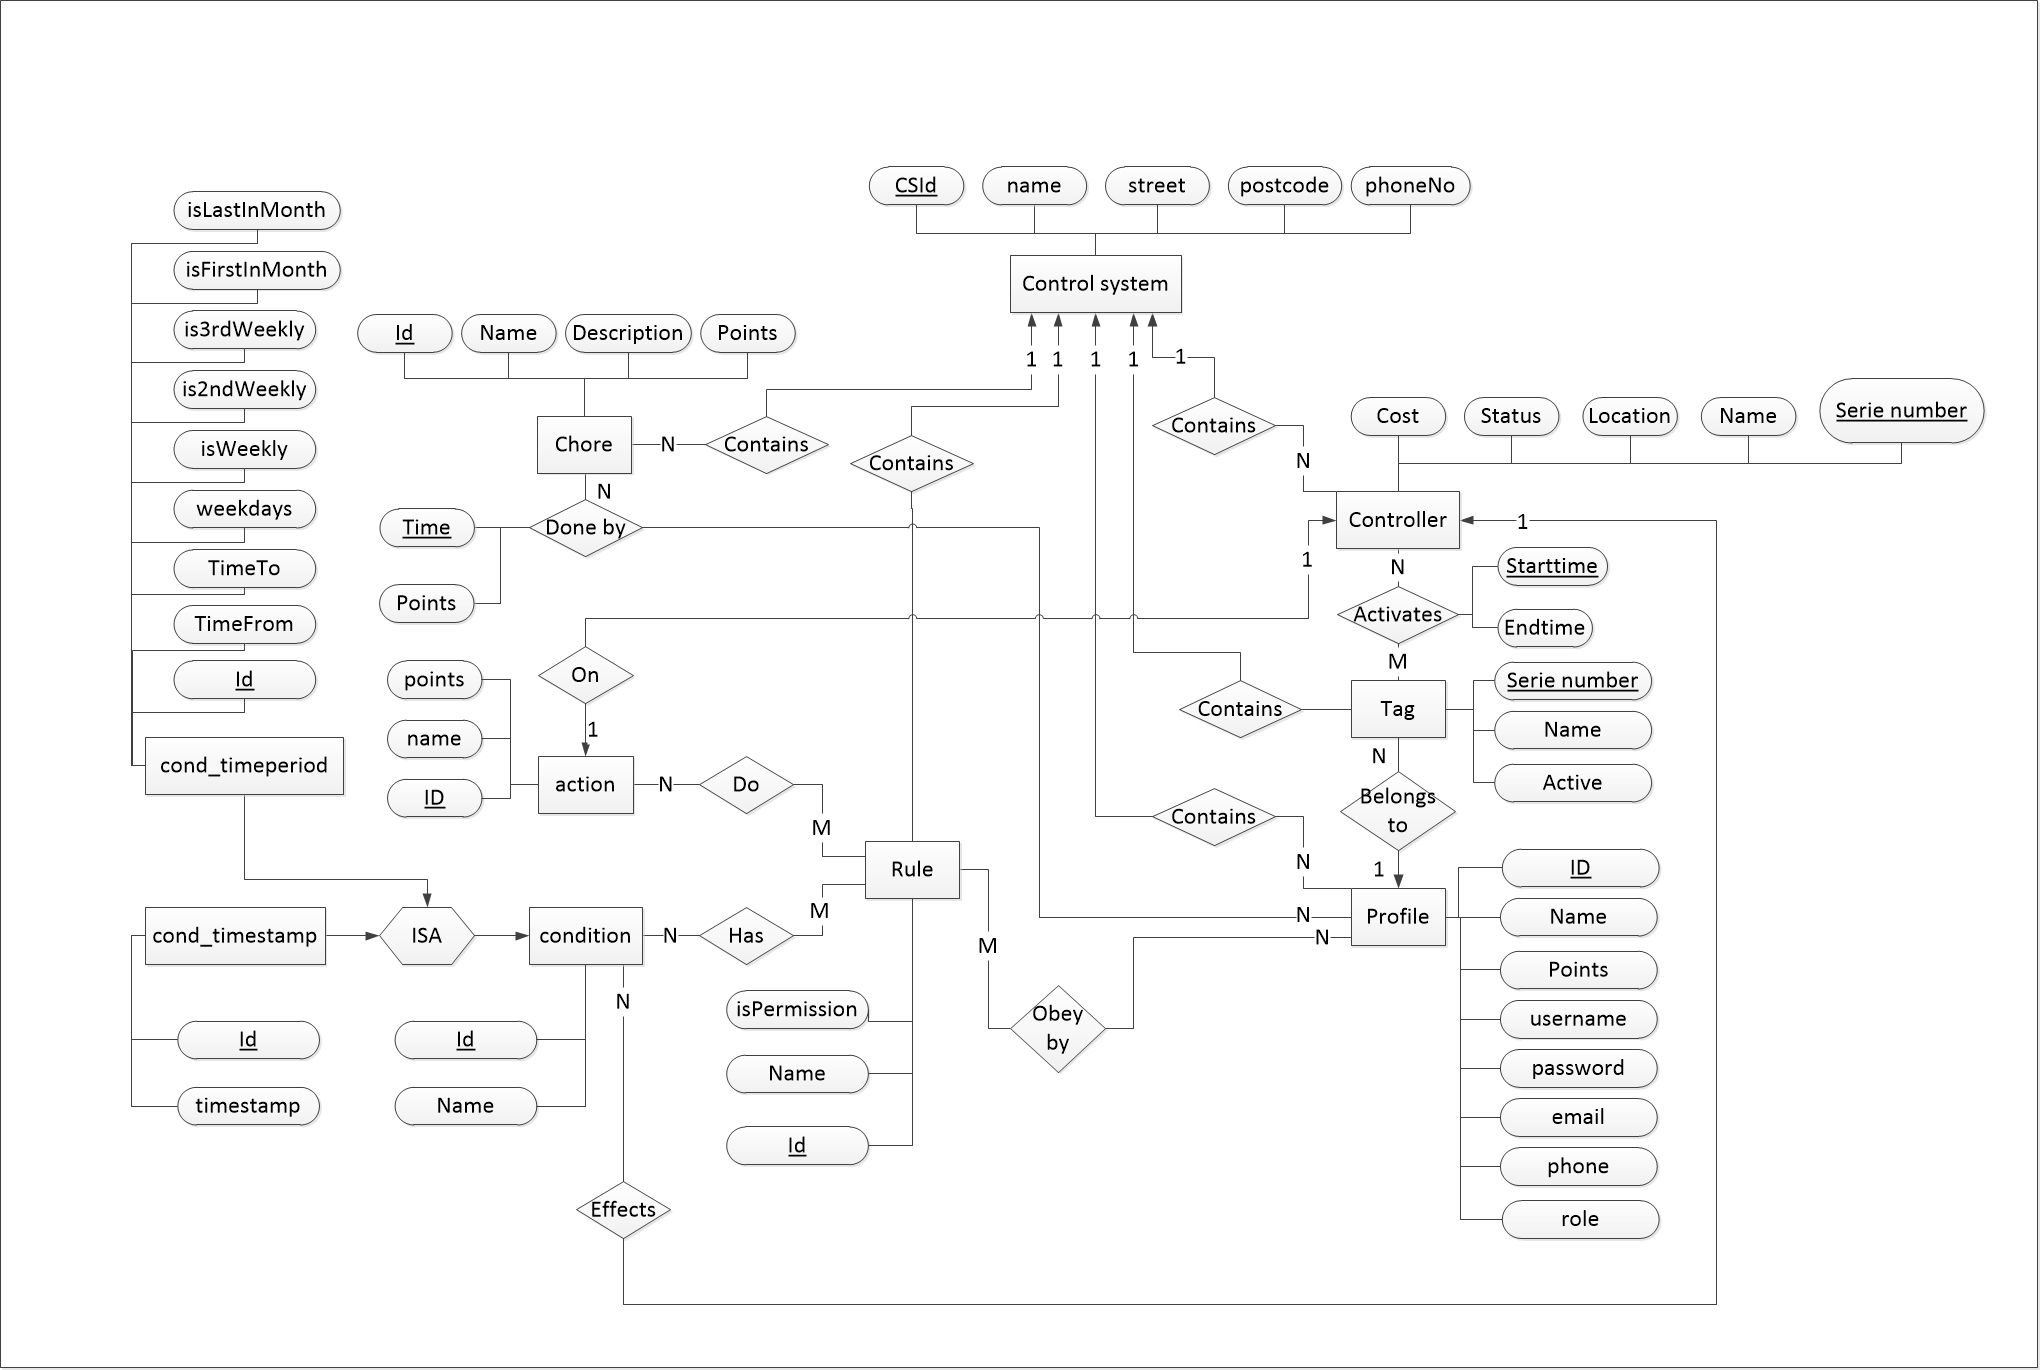
\includegraphics[width=1.00\textwidth]{images/ERdiagram.jpg}
	\caption{ER schema of the database design}
	\label{fig:ERdiagram}
\end{figure}

In the database design it should be noticed that Permission is absent. The reason is for every permission that could be made then there is an equivalent rule. Therefore the data representation of Permission is the same as Rule. However, on the website the two should be represented differently and so the attribute \texttt{isPermission} have been add to Rule which will differentiate the two.

Another observation in the design is the condition of a rule. The condition can be one of three representations. The first is the simplest because it is just the Condition. The second is Condition and a timestamp which is the \texttt{cond\_timestamp} in the design in \ref{fig:ERdiagram}. The last representation is Condition, a time period, and a representation of when it is valid, which in the design is \texttt{cond\_timeperiod}. 
 It is the name of the condition which distinguishes the representation that should be used. If the name is \texttt{Timestamp} it should be cond\_timestamp, if it is \texttt{Timeperiode} then it is cond\_timeperiod and any other name it is only the Condition. \fixme{Til sidst er navne stadig TimeStamp og TimePeriod}

After the design in the ER-schema has been completed it was implemented into a MySQL database.  

\section{Implementation}

The design from figure \ref{fig:ERdiagram} has been implemented in a MySQL database and the result can be found in figure \ref{fig:databaseDiagram}. In the implementation of the database redundancy and anomalies is to be avoided and null values reduced. 
The mapping from the ER-schema to a relations representing in the database is basic mapping according to the relations $1:1$, $n:1$, $n:m$ except for Condition which decision is clarified in the following section\citep{DatabaseKilde}. 

\begin{figure}
	\centering
		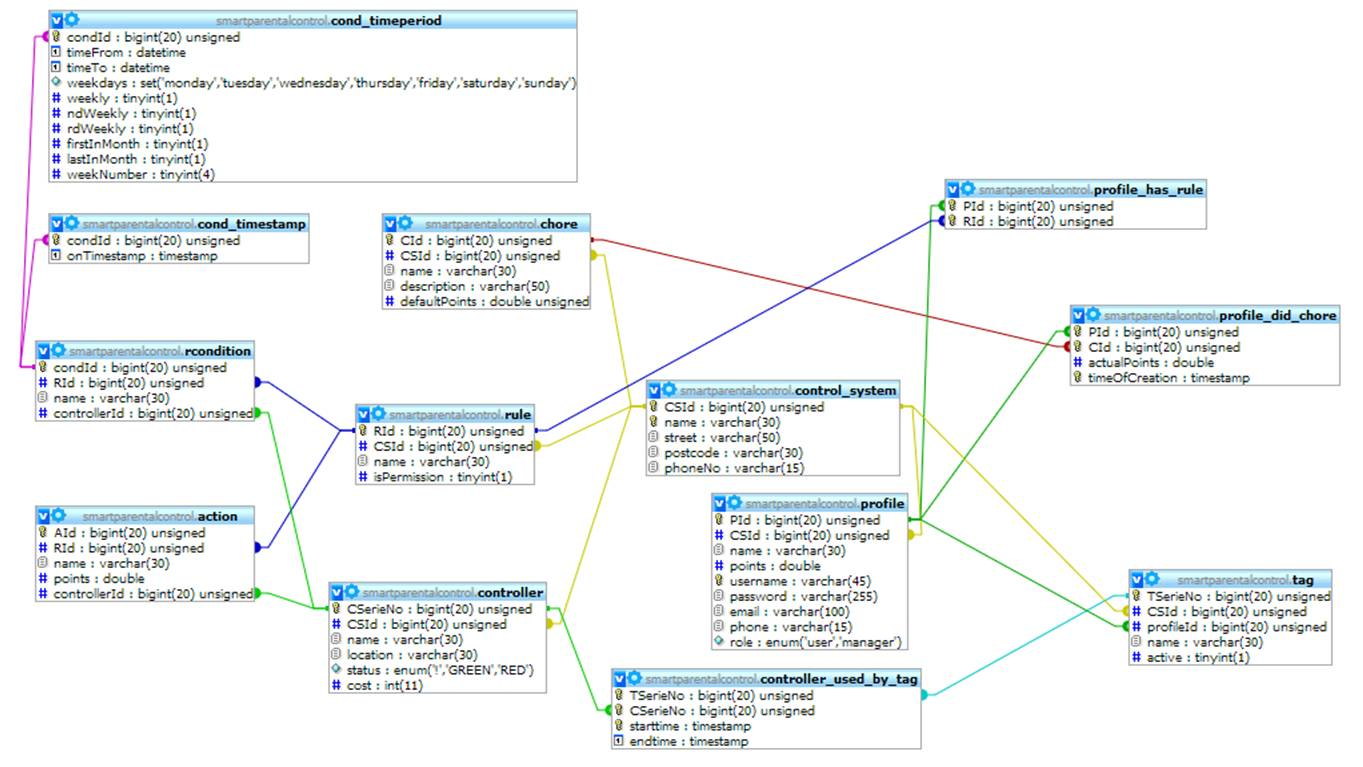
\includegraphics[width=1.00\textwidth]{images/databaseDiagram.jpg}
	\caption{The Database implementation}
	\label{fig:databaseDiagram}
\end{figure}

\subsection{Mapping of Condition}
\label{subsec:mappRule}
%sql or diagram
The relational modeling of Condition is more advanced because it uses generalization and as such there are a implementation choice that should be made. There are four typical method of how to deal with generalization and a solution of using each method is described below \citep{DatabaseKilde}.

\begin{description}
	\item[Using main classes,] then Condition is split up into three tables rcondition, cond\_timestamp and cond\_timeperiod where the all attributes in Condition are repeated in each table. An disadvantage of using this method is in querying because it is possible to go though all three before finding the wanted tuple.
	\item[Using partitioning,] there there are three tables rcondition, cond\_timestamp and cond\_timeperiod. The common attributes are in Condition and via an id the possible additional data can be found in either cond\_timestamp or cond\_timeperiod.
	\item[Using full redundancy,] it is much like the first but where all conditions from cond\_timestamp and cond\_timeperiod are also represented in Condition, without the additional data. As the name suggest this causes redundancy which is best avoided.
	\item[Using single relation,] so there will be a single table with all attributes from condition, cond\_timestamp and cond\_timeperiod. This will increase the number of null values. 
\end{description}

As the \ref{fig:databaseDiagram} suggest the partitioning option is used in our implementation since it does not causes any redundancy or null values and it is easier to search for conditions compared to using the main classes. However, using partitioning there will be some challenges in making the functions to insert, update and get data about the rules, as will be explained in section \vref{subsec:dbRule}.\\\\


There have also been made an important decision about how to deal with deletion of tuples from the essential tables and this is explained in the following section.
 
\subsection{Deleting in the database}
%delete cascade
When a tuple in one of the tables control\_system, profile, tag, controller, chore, and rule should be deleted it will likely affect one of the other tuples from another table because of the foreign keys. We have made an intentionally decision to use \texttt{ON DELETE CASCASED} with all foreign keys, because in any case when deleting a tuple from the essential tables its history is irrelevant and should be deleted.


As an consequence of this decision if a control system is deleted then every profile, tag, controller, chore, and rule which is connected to control system will be deleted, so this should be used with care. 
If a profile is deleted then this profile's tags will be deleted including all of its history, such as when the tag have been used to activate the controllers, or when the user have done a chore.
 So it is very important that when one of the important tuples are to be deleted then it will not be regretted later.  \\\\

However, for anything to be added, updated or deleted by the user the website need a connection to the database which happen through the class MySQLHelper. 

%sql Helper class
\subsection{MySQLHelper class}
The website and API for the controllers connect to the database by using a PHP class MySQLHelper, which establish a connection and send queries to it. The class have a construct and destruct that respectively establish the connection and close the connection to the database. The queries goes also through this class in at least one of these method:

\begin{description}
	\item[insertInto] this make a SQL string to insert into the database.
	\item[update] this make a SQL string to update data in the database.	
	\item[delete] this make a SQL string to delete data in the database.
	\item[query] this make a SQL query string.
	\item[executeSQL] this send the query to the database and return the result. All of the above uses this method.
\end{description}
  
It is also possible to control the transactions through this class by disabling the auto-commit of transactions and then manually commit when it is necessary. \\\\

This class is used by several functions that are connected to the website or API and in the following sections we present a code sample for updating one of the simpler object and how to update rules. 

\subsection{Functions to simple Update}
%if someday our repport gets to long this can be cut out or reduced
To insert, update or delete in one of the tables: control\_system, profile, tag, controller or chore, one of the functions \texttt{simpleInsertIntoDB}, \texttt{simpleUpdateDB} or removeObjectFromDB is used. They all uses some classes that have been made to rape the data of a tuple from each table and the classes are used alike in the function. The functions are build in a similar way and therefore only simpleUpdateDB will be presented. One thing that must be pointed out about using simpleUpdate is that if a variable is not to be updated then it should be null in the class, with only one exception which is the primary key. 

%Since it is possible that not all of the class variable should be updated in the database and therefore these values in the class must be null except for the primary key.
In code sample \ref{code:simpleUpdate} is a shorted version of the function \texttt{simpleUpdateDB}.  
First the dynamic typing of PHP is used to discover which class type the input is and then parts of the SQL string can be made,see line $9-40$\fixme{check line no}. Then the string followed by the sql command SET in the update statement is made in the control structure, see line $15-36$\fixme{check line no}. 
Finally the result after sending the executing the update statement can be a Boolean value which indicate success or an error code contained in an array from which a error message is returned, see line $41-49$\fixme{check line no}.

\begin{lstlisting}[language=PHP, label=code:simpleUpdate, caption=simpleUpdateDB code sample]
function simpleUpdateDB($object)
	{
		global $theColumns;
		global $theTables;
		$table;
		$columnValue;
		$where;

		switch (get_class($object))
		{ 		
		case 'Controller':
			$table=  $theTables['Controller']; //get controllers tablename
			$columstemp= $theColumns['Controller']; //get controllers columns in array
			$where = $columstemp[0] . " = " . $object->CSerieNo;
			$columnValue = "" ;
			if($object->name != null)
			{
				$columnValue .= $columstemp[2] . " = '" . $object->name . "'";
			}
			if($object->location !== null) 
			{
				if($columnValue != "")
				{
					$columnValue .=  ", ";
				}
				$columnValue .=  $columstemp[3] . " = '" . $object->location . "'";
			}
			
			if($object->cost != null)
			{
				if($columnValue != "")
				{
					$columnValue .=  ", ";
				}
				$columnValue .=  $columstemp[5] . " = " . $object->cost;
			}
			break;
			/*similar switch cases exist for control_system, profile, tag, controller or chore*/
			default: 	return;
		}
		$resultValue = $db->update( $table, $columnValue, $where); //update the 
		if(is_bool($resultValue))
		{ 
			return $resultValue;
		}
		elseif(is_array($resultValue))
		{
			return sqlErrorMessage($resultValue[1]);
		}
		return null;
	}	
\end{lstlisting}

Inserting and updating a rule are different from the others and more complicated so its functions are explained in the following section. 
%control system, profiles, tags, controller, chores, rules

\subsection{Function working with Rule}
\label{subsec:dbRule}


As stated previously in mapping of a rule in \vref{subsec:mappRule}, there will be some challenges to make the insert and update functions. This is partly due to the fact that condition data is one of three alternative: condition, condition plus timestamp or condition plus timeperiod as was explained in \vref{sec:DBdesign}.
In update it is also a challenge that each condition and action can be removed, add or updated which all should be handled together and this will be explained further in this section. 

As with the simpler updates this also uses some data rapping classes \texttt{Rules}, \texttt{Action} and \texttt{Condition}. In the class Condition there is a variable \texttt{arrayOfRestAttributes} which is an array with the attributes from either cond\_timeperiod or cond\_timestamp.

The function to update a rule is called editRule and it also used some other function as described below:

\begin{description}
	\item[addAction] from a rule id and a object of type Action it adds an action to the rule.
	\item[editAction] from a object of type Action it updates the attributes in the database.   
	\item[addCondition] from a rule id and a object of type Condition adds a condition to the rule.
	\item[editcondition] from a object of type Condition it updates the attributes in the database.   
\end{description}

The editRule has three inputs a Rule object, an array with Condition objects, and an array with Action objects. Updating the rule table is like the simple updates of the other tables and therefore it will not be represented in the code sample. After the rule have been updated each condition and action must also be updated. 

However, when updating an action and especially a condition the changes can have different characteristics as listed below.

\begin{itemize}
	\item a new condition or action is add.
	\item a condition or action need to be deleted.
	\item an existing condition or action is to be updated with no structural change in the database.
	\item an existing condition or action is to be updated but with a structural change in the database.
\end{itemize}

With a structural change it is meant that the name of the condition or action has been changes and this change can influence e.g. whether cond\_timeperiod or cond\_timestamp should be used. As a result it have been decided that in this case the old condition should be deleted and the new be added anew. 

The code sample in \ref{code:UpdateRules} is from the update handling of condition and the it is similar to handle the actions. First the old conditions id are need such that they can be compared to the ids of the Condition objects from the array \$arrayOfCondition, see line $2$\fixme{check line no}. 
Then foreach old condition id we will look thourgh the new id and if it found and the name are not to be changed then we call editcondition with the updated condition object and remove this object from the array of condition, see line $4-20$\fixme{check line no}. 
From line $22-26$\fixme{check line no} it is shown that the tuple with the old id is removed if no match was found among conditions in the array or if a match was found but the name are to changed. Now all the condition that was intended to be deleted is gone and finally the remain objects is then add or re-add from the array with addCondition, see line $28-40$\fixme{check line no}.


\begin{lstlisting}[language=PHP, label=code:UpdateRules, caption=editRule code sample]
//SELECT condId AS id FROM rcondition WHERE RId = ($ruleData->RId)
$CondIdResult = $db->query($theColumns['Rcondition'][0].' AS id', $theTables['Rcondition'], $theColumns['Rcondition'][1] . " = " . $ruleData->RId );
				
	while($row = mysqli_fetch_assoc($CondIdResult))
	{
		$StillExists = false;
		foreach($arrayOfCondition as $key => $cond)
		{
			if($row['id'] == $cond->condId && $cond->name == null)				//edit the condition in db
			{
				$StillExists = true;
				$tempresults = editCondition($cond);
				unset($arrayOfCondition[$key]);
				if(is_string($tempresults))
				{
				//if not bool then it is an error message
					return $tempresults;
				}
			}	
		}
		//row id is not among the updated condition or cond_name not null so delete 
		if(!$StillExists)
		{
			$db->delete($theTables['Rcondition'], $theColumns['Rcondition'][0] . " = " .$row['id']);
		}
	}
	//add the remaining condition to db
	if($arrayOfCondition != null )
	{
		foreach($arrayOfCondition as $cond)
		{
			//if a new condition should be added then make condition here
			$tempresults = addCondition($ruleData->RId, $cond);
			if(is_string($tempresults))
			{
			//if not bool then it is an error message
				return $tempresults;
			}
		}
	}
\end{lstlisting}



